\chapter{実装}
\label{implementation}

本章では本研究における実装環境,提案手法の実装,提案手法の評価に用いるデータセットについて述べる.
その後実験に用いたハイパーパラメータ,実装における留意点について解説を行う。

今回は大きく3つの比較実験を行う。



\section{実装環境}



本研究において利用した実装環境を Table 4.1 に示す. 提案手法の実装は Pytorch 及
を用いた.  PyTorch, Chainer は計算グラフの自動微分ライブラリであり, 深層ニューラ
ルネットワークの研究や開発にも用いられる.
Pytorchを用いた理由は実装コストが低く研究領域に従事できるところにある。



\begin{table}[htbp]
    \begin{center}
        \caption{本研究の実行環境}
        \begin{tabular}{l*{2}{c}r}
        ソフトウェア              & バージョン \\
        \hline
        Python            & 3.6.2 or above \\
        CPU               & intel core i7 \\
        Tensorflow        & 2.1.0-rc0 \\
        PyTorch           & 6 \\
        \end{tabular}
    \end{center}
\end{table}



\section{比較データ}

他の活性化関数と適当に比較するために、以下の条件を比較して実験を行う。
\begin{itemize}
    \item ラーニングレート
    \item 初期値、
    \item レギュラライザー(l1ノルムなど)
    \item optimizer
    \item テストデータ
\end{itemize}
既存のものと比較している
\subsubsection{ラーニングレート}

\subsubsection{初期値}
初期値は
\subsubsection{レギュラライザー}
レギュラライザーはL1ノルム, L2ノルム等の比較ができる。
\subsubsection{optimizer}
\subsubsection{テストデータ}
各テストデータの特徴を以下の表にまとめる。データセットには出力の形式が存在し、多くの問題は「分類」もしくは「回帰」の二つに分類される。


\begin{table}[htbp]
    \begin{center}
        \caption{実験のデータセットの名称}
        \begin{tabular}{l*{2}{c}r}
        データセット名      & 出力層 & 出力の形式 \\
        \hline
        iris            & 3  & 分類 \\
        MNIST               & i10 & 分類  \\
        wine        & 13 & 分類 \\
        住宅の価格           & 6 & 回帰 \\
        健康の状態           & 6 & 回帰 \\
        膵臓癌           & 6 & 回帰 \\
        \end{tabular}
    \end{center}
\end{table}



\section{実装手法}

各データセットにおける中間層は以下のパラメータで固定した。


\begin{figure}[hbtp]
    \begin{center}
        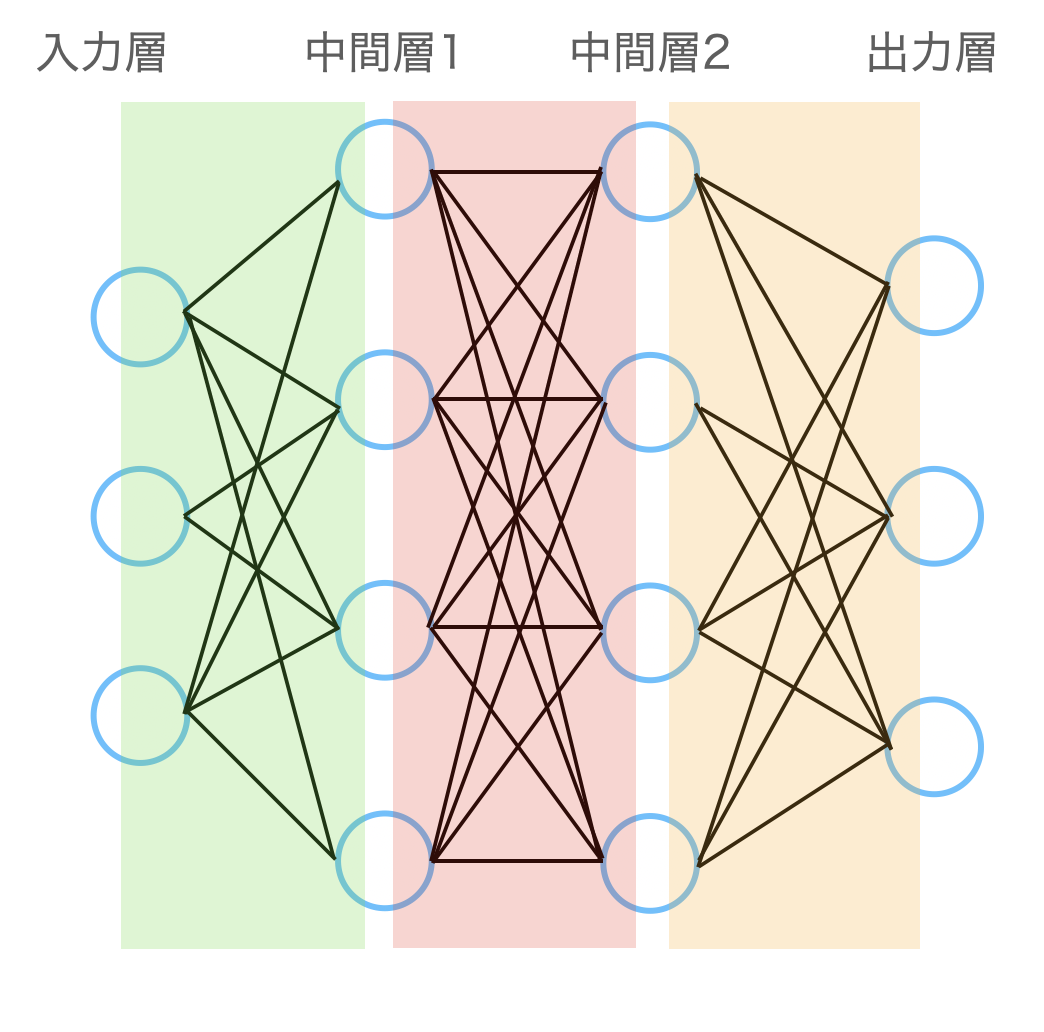
\includegraphics[width=10cm]{asset/neural_network1.png}
            \caption{活性化関数の形}
            \label{neural_network1}
    \end{center}
\end{figure}



\section{活性化関数}



\section{実装における留意点}
本研究における提案手法を実装する際に留意する必要のある点を述べる.
一つは勾配が消失してしまった場合の処理である。

\section{}

%%% Local Variables:
%%% mode: japanese-latex
%%% TeX-master: "../bthesis"
%%% End:
